\section{Linearização do Modelo}

A implementação de controle preditivo em hardware embarcado 
exige soluções computacionalmente menos custosas, 
devido ao baixo poder de processamento dos microcontroladores. 
Isso favorece a utilização de modelos lineares, dada a simplicidade 
na minimização de funções quadráticas.

\vspace{1em}
Para reduzir o custo computacional do controle, 
utilizaremos a linearização por meio de séries de Taylor 
em torno de $\omega_0$ e $v_0$.

\vspace{1em}
Assumiremos que o centro do referencial está localizado no 
centro geométrico do robô, e que sua orientação permanece 
fixa em 0 graus em relação ao eixo $x$.

\begin{figure}[h]
    \centering
    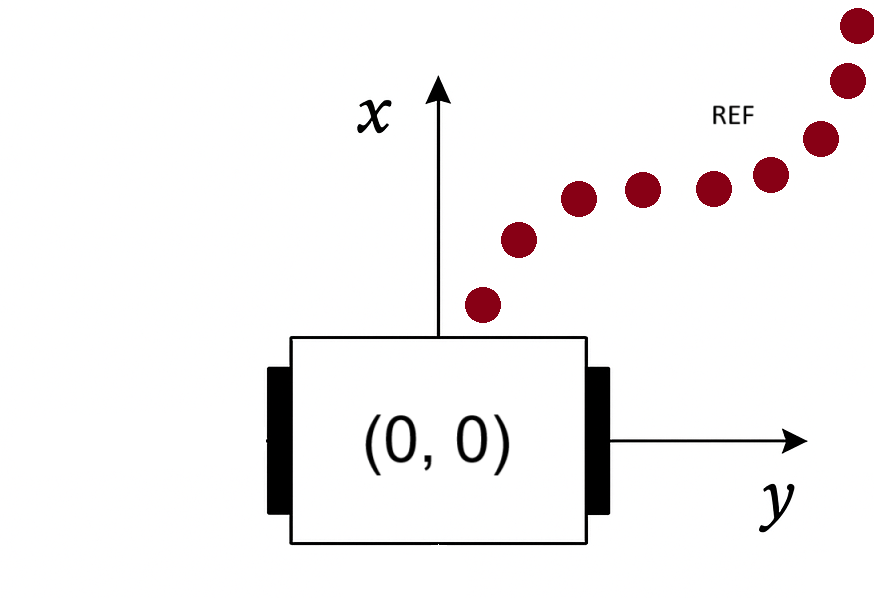
\includegraphics[width=0.5\textwidth]{figures/robot_reference.png}
    \caption{Referencial do robô}
    \label{fig:robot_reference}
\end{figure}

Utilizando a aproximação por séries de Taylor:

\[
x = x_0 + \frac{\partial x}{\partial v} \bigg|_{v_0} \Delta v + \frac{\partial x}{\partial \omega} \bigg|_{\omega_0} \Delta \theta
\]
\[
y = y_0 + \frac{\partial y}{\partial v} \bigg|_{v_0} \Delta v + \frac{\partial y}{\partial \omega} \bigg|_{\omega_0} \Delta \theta
\]

Assim, o modelo cinemático definido na Equação~\ref{eq:cinematic_velocity} 
pode ser representado em $(x, y)$ como:

\begin{equation}
\begin{cases}
x \approx v_0 \cos(\omega_0) + \cos(\omega_0) \Delta v - v_0 \sin(\omega_0) \Delta \theta \\
y \approx v_0 \sin(\omega_0) + \sin(\omega_0) \Delta v + v_0 \cos(\omega_0) \Delta \theta
\end{cases}
\end{equation}

Considerando os valores numéricos com $\omega_0 = 0$, temos:

\begin{equation}
\begin{cases}
\dot{x} \approx v \\
\dot{y} \approx v_0 \theta \\
\dot{\theta} = \omega
\end{cases}
\qquad
\Rightarrow
\qquad
\begin{cases}
x \approx s \\
y \approx s_0 \theta \\
\end{cases}
\label{eq:linearized_model}
\end{equation}

É possível observar que ao linearizar o modelo, 
acontece um desacoplamento entre as variáveis de estado,
resultando em em uma relação direta entre a velocidade linear $v$ e a posição $x$,
e entre a velocidade angular $\omega$ e a posição y. Simplificando significativamente
 a relação entre a posição $\mathbf{q}$
e as entradas de controle $\mathbf{u}$.